\begin{center}

\begin{tikzpicture}[font=\small,overlay,
mycirclex/.style={draw, circle, minimum size=1.0em, inner sep = 0.2mm}, 
mydiamond/.style={draw, diamond, minimum size=0.78em, inner sep = 0mm}, 
myrectang/.style={draw, rectangle, minimum size=0.60em, inner sep = 0mm}, 
>=stealth]

\definecolor{mygreen}{rgb}{0, 0.7, 0}
\definecolor{myyellow}{rgb}{0.8, 0.6, 0}

\def\colx{black}
\def\cola{red} 
\def\colb{blue}
\def\colc{violet}
\def\cold{cyan} 
\def\cole{myyellow}
\def\colf{brown}


\def\len{1.8cm}

% G1
\begin{scope}[local bounding box=bbox, xshift=-6.4cm, yscale=1.2]
\path<7-> node[mycirclex] (v1) at (1.0 * \len, 0) {$s$};
\path<7-> node[mycirclex] (v2) at (2.0 * \len, 0) {$a$};
\path<7-> node[mycirclex] (v3) at (3.0 * \len, 0) {$b$};
\path<7-> node[mycirclex] (v4) at (4.0 * \len, 0) {$c$};
\path<7-> node[mycirclex] (v5) at (5.0 * \len, 0) {$d$};
\path<7-> node[mycirclex] (v6) at (6.0 * \len, 0) {$t$};

\path<11-> [draw, \cold, ->, line width=0.122cm, bend left = 50] (v1) to (v2);
\path<11-> [draw, \cold, ->, line width=0.122cm, bend left =-20] (v2) to (v3);
\path<11-> [draw, \cold, ->, line width=0.122cm, bend left =-20] (v4) to (v5);
\path<11-> [draw, \cold, ->, line width=0.122cm, bend left = 50] (v5) to (v6);
\path<11-> [draw, \cold, ->, line width=0.122cm] (v3) -- (v4);

\path<10-> [draw, \colc, ->, line width=0.122cm, bend left = 30] (v1) to (v4);
\path<10-> [draw, \colc, ->, line width=0.122cm] (v4) -- (v5);
\path<10-> [draw, \colc, ->, line width=0.122cm] (v5) -- (v6);

\path<9-> [draw, \colb, ->, line width=0.122cm] (v1) -- (v2);
\path<9-> [draw, \colb, ->, line width=0.122cm] (v2) -- (v3);
\path<9-> [draw, \colb, ->, line width=0.122cm, bend left = 30] (v3) to (v6);


\path<8-> [draw, \cola, ->, line width=0.052cm] (v1) -- (v2);
\path<8-> [draw, \cola, ->, line width=0.052cm] (v2) -- (v3);
\path<8-> [draw, \cola, ->, line width=0.052cm] (v3) -- (v4);
\path<8-> [draw, \cola, ->, line width=0.052cm] (v4) -- (v5);
\path<8-> [draw, \cola, ->, line width=0.052cm] (v5) -- (v6);

\path<7-> [draw, \colx, ->, line width=0.02cm] (v1) -- (v2);
\path<7-> [draw, \colx, ->, line width=0.02cm] (v2) -- (v3);
\path<7-> [draw, \colx, ->, line width=0.02cm] (v3) -- (v4);
\path<7-> [draw, \colx, ->, line width=0.02cm] (v4) -- (v5);
\path<7-> [draw, \colx, ->, line width=0.02cm] (v5) -- (v6);

\path<7-> [draw, \colx, ->, line width=0.02cm, bend left = 50] (v1) to (v2);
\path<7-> [draw, \colx, ->, line width=0.02cm, bend left = 50] (v5) to (v6);
\path<7-> [draw, \colx, ->, line width=0.02cm, bend left = 30] (v1) to (v4);
\path<7-> [draw, \colx, ->, line width=0.02cm, bend left = 30] (v3) to (v6);

\path<7-> [draw, \colx, ->, line width=0.02cm, bend left =-20] (v2) to (v3);
\path<7-> [draw, \colx, ->, line width=0.02cm, bend left =-30] (v2) to (v3);
\path<7-> [draw, \colx, ->, line width=0.02cm, bend left =-40] (v2) to (v3);
\path<7-> [draw, \colx, ->, line width=0.02cm, bend left =-50] (v2) to (v3);
\path<7-> [draw, \colx, ->, line width=0.02cm, bend left =-20] (v4) to (v5);
\path<7-> [draw, \colx, ->, line width=0.02cm, bend left =-30] (v4) to (v5);
\path<7-> [draw, \colx, ->, line width=0.02cm, bend left =-40] (v4) to (v5);
\path<7-> [draw, \colx, ->, line width=0.02cm, bend left =-50] (v4) to (v5);


\path<7-> node at (1.5 * \len, 0.17cm) {$2n$};
\path<7-> node at (2.5 * \len, 0.17cm) {$2n$};
\path<7-> node at (3.5 * \len, 0.17cm) {$2n$};
\path<7-> node at (4.5 * \len, 0.17cm) {$2n$};
\path<7-> node at (5.5 * \len, 0.17cm) {$2n$};

\path<7-> node at (1.4 * \len, 0.62cm) {$n$};
\path<7-> node at (5.6 * \len, 0.62cm) {$n$};
\path<7-> node at (2.5 * \len, 0.96cm) {$n$};
\path<7-> node at (4.5 * \len, 0.96cm) {$n$};

\path<7-> node at (2.5 * \len, -0.65cm) {$n\times 1$};
\path<7-> node at (4.5 * \len, -0.65cm) {$n\times 1$};
\end{scope}


\end{tikzpicture}
\end{center}
